\section{Introduction}
so, need to figure out what the general order of this paper will be. let's try the following: \\
1.0 introduction \\
2.0 related work \\
3.0 Short overview of components in stereo network \\
  3.1 psmnet and stereo estimation networks \\
  3.2 mathematics of stereo 3D reconstruction \\
  3.2 pointnet and pointnetworks \\
4.0 general steps of spnet (stereo point net) \\
  4.1 stereo estimation (performance, results) \\
  4.2 stereo 3d reconstruction (performance, results) \\
  4.3 stereo point net (procedure, modifications, performance) \\
5.0 results of stereo point net \\
R. references \\
A. appendices(?) \\

\subsection{Problem / Motivation}
The field of artificial intelligence has exploded in recent years, in part due to the usage of convolutional neural networks and the usage of graphics processing units, GPU's. This has enabled further research into systems that can quickly understand their surroundings, having applications to many processes, one of which is autonomous driving. The subfield of autonomous driving has seen great success in the application of camera data for 2D localization. However, driving being a process that requires 3D knowledge, the usage of lidar has followed the growth of this subfield. To its credit, lidar is a technology with multiple benefits: a lidar scan is precise, works outside, works in darkness, and provides immediate metric information about the world. Unfortunately, lidar sensors also have the disadvantage of being expensive relative to the amount of information they output when compared to something like a camera image [CITATION NEEDED XX], have relatively slow refresh rates (on the order of 10 Hz for a commercial Velodyne VLP-16), requires active sensing and thus may create a high degree of noise if there are many sensors in the same area, and may not work well with some reflective surfaces, even if they are close (such as a car window not directly perpendicular to the incident laser ray). Despite this, and despite lidar being a worthy technology of use, this paper seeks to explore an alternative technology, stereo vision, to estimate the 3D positions of objects. 

There are some interesting benefits that may be gained with stereo vision: stereo cameras are relatively cheap for the amount of information they provide [CITATION NEEDED XX], intuitively mimics the way that humans already perceive and navigate their world, is a passive sensor that does not interfere with other sensors, and have a high refresh rate (dependent on the camera system, but 30 Hz, "frames per second", is around the lowest value for any camera). Of course, using a stereo vision system is not without downsides, which can include inability to function at night without adequate lighting, difficulty understanding large texture-less surfaces, and when used to estimate position a squared error relationship to distance. This last points simply means that as the distance of an estimated point increases, the error of that value increases quadratically [CITATION NEEDED XX]. 

With these pros and cons in mind, this paper takes the position that stereo vision can provide practical benefits to robotics and autonomous systems under the right conditions. Using stereo vision to estimate 3D locations of objects, specifically cars, is believed to be somewhat competitive with lidar.


\subsection{Requirements}
In order to develop a stereo-based 3D estimation algorithm and conduct a performance comparison, there are multiple needs that must be met. The very first need that must be met is a dataset that contains all the necessary information for a lidar-based network to detect objects, as well as a stereo-based network. For this reason the KITTI dataset, a well-known and actively used benchmark, was selected as the source of data to compare the two technologies.

% ==============================================================================
\section{Related Work}
\subsection{Stereo Vision Networks}
Stereo disparity maps, which are built by the comparing the pixel distance between two similar regions of two images, have existed before the implementation of artificial intelligence to create them. Famously, \cite{scharstein_taxonomy_2002} gave a taxonomy and categorization of the various aspects of stereo vision. Out of this paper, the four main parts of conducting stereo vision have been defined as follows: 

\begin{enumerate} \itemsep=-0.5em
    \item matching cost computation
    \item cost (support) aggregation
    \item disparity computation/optimization; and
    \item disparity refinement
    
\end{enumerate}

(xx include here information about psmnet!!!)
(xx include here info about traditional stereo vision)
(xx include here info about competitive, ai-based stereo networks)




\subsection{3D estimation with Stereo Disparity Maps}
There is a surprisingly low amount of public research on stereo vision for use with 3D localization. \cite{li_stereo_2019} created an RCNN-based approach that currently performs best in class on the KITTI dataset, although achieving 59'th place when also compared against networks that use lidar. This paper also cites other works, such as "3DOP" by \cite{chen_3d_2016}. However, some prior information is encoded into the calculation before using regression to estimate object pose, including height above ground, object size priors, and "depth informed features", while our paper does not provide this information to the network beforehand.

A recent development has been published since the start of this paper, by Wang et. al. In their paper, "Pseudo-LiDAR from Visual Depth Estimation" \cite{wang_pseudo-lidar_2019}, the authors took an extremely similar approach to this paper. Their pipeline / steps, outlined below in Figure \ref{wang_pipeline}, was to take a stereo image pair, generate a disparity map via Pyramid Stereo Matching network, convert it to a "pseudo-lidar" scan, and extract 3D bounding box estimations via Frustum Pointnet. \\

\begin{figure}[h] % h = "approx here", {h,t,b}
    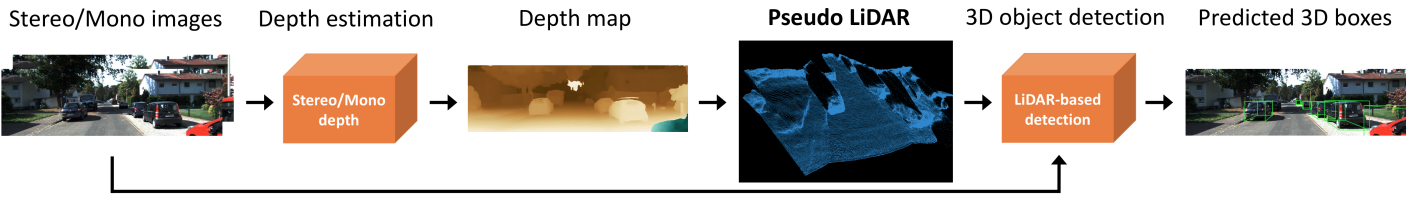
\includegraphics[width=1\textwidth]{../media/wang_pipeline.png}
    \caption{Pipeline of the Pseudo-Lidar estimation network. Stereo (or mono) image data is used to create a disparity map, which is converted to lidar, and is then used by a 3D detector to estimate 3D bounding boxes.}
    \label{wang_pipeline} %label goes last
\end{figure}

In their paper, the authors argue that within a short distance, up to 30 meters away, stereo vision performs competitively with lidar.

\subsection{3D Estimation with Lidar}
Performing 3D estimation and localization with lidar has been a focus for a large portion of the field, and with good reason. Thus, there are many papers which focus on using lidar sensor capabilities to estimate 3D bounding boxes, to varying degrees of success. \cite{qi_frustum_2017} paper, currently one of the best performing networks, forms a part of the work of this research paper as well. 

\subsection{3D Reconstruction with Stereo Data}
So, i'm having trouble finding information about 3D reconstruction, and i think it may be because i'm using the wrong terminology. almost invariably, 3d reconstruction is used to describe the process of taking photos of an object with multiple cameras to then creating a 3D model. instead, i am trying to obtain a point cloud from a stereo image. unfortunately, i think this may either be a rare or unpopular task... doesn't seem like there's a lot of people doing it. i'm gonna make a small list of all the places that i find references about stereo-point cloud conversion: 

%\url{https://www.youtube.com/watch?v=ujm3TKfVarQ} \\
%\url{https://www.researchgate.net/post/3D_reconstruction_from_stereo_images_the_point_clouds_seem_to_be_warped_and_curved_towards_the_edges_of_the_image_why}\\
Really there just isn't much to use in the way of "research". So, will instead cover the "traditional" methods. For one, will cite \cite{szeliski_computer_2010}, a very helpful book for understanding stereo correspondence as well as reconstruction.






% ==============================================================================
\section{Development of 3D Estimation Network}
At this point, we can start talking about how you have modified all the different networks to make them work for you. you should definitely catalog your troubles with each one. pwe can talk about this in depth. 

\subsection{Modification of Pyramid Stereo Matching Network}
The first task in creating a network that can take a stereo image pair and generate 3D bounding boxes, as described in figure xx above, is to have the capability of taking a stereo image pair and creating a 2.5D disparity map. To that end, a best-in-class disparity generation algorithm was searched and was selected to be the Pyramid Stereo Matching Network. Pyramid Stereo Matching Network was published by Jia-Ren Chang and Yong-Sheng Chen in March 2018. This network takes a deep learning approach to generating disparity maps from a pair of images. The network itself is near the top of the state of the art, and achieves this by the architecture of its network. (xx architecture and style need to be elaborated upon in the "related work" section). The openly-available repository provided a foundation to start on towards making a compact, easy-to-use function. 

the original evaluation code that was given was straightforward. i had great success in testing it out right away. Of course, there were some usual delays with making sure the correct packages were installed. additionally, the network was adapted to run in python3. as has been stated before, this project has placed a great focus on ensuring the future usability of the code, and so python 3.x was used. any deprecated functionality was manually changed. 

after the initial evaluation, i set about to training the network from the ground up. i first pretrained the network from scratch using the Freiburg dataset, then further pretrained it on the Middlebury dataset. finally, i finetuned the network by training it on the KITTI stereo dataset, which contains similar but not identical scenes that are seen in the 3d object detection dataset. 



\subsection{Development of Stereo 3D Reconstruction Function}
texthere

\subsection{Modification of Frustum Point Net}

Frustum Pointnet, being originally written for Python 2, needed to undergo some minor adaptations while being modified for usage with Python 3. For example, several modules and functions were deprecated or modified, and so had to be properly adapted. There are also two actively maintained versions of the frustum Pointnet code. as explained in the original paper [xx], there are two versions of the FPNet model: the first which uses standard Tensorflow libraries, and the second which uses custom Tensorflow operators that must be compiled. For the purposes of this paper, version 1 was used and will be the default version unless otherwise noted. 

In order to transition from using the provided pretrained model and preprocessed data to self-made preprocessed and trained data, a set of steps and "paths" were created to clarify what was happening in each step and set of "runs". As shown below in Figure \ref{fp_paths}, there are various 

\begin{figure}[h] % h = "approx here", {h,t,b}
    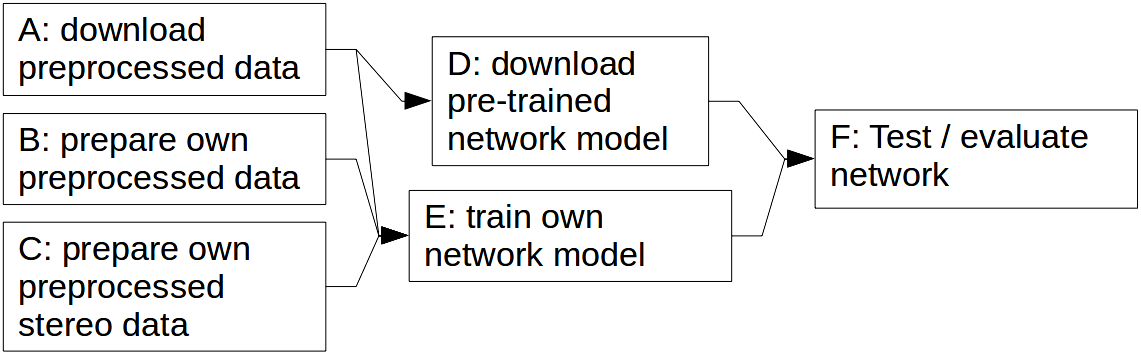
\includegraphics[width=1\textwidth]{../media/fpnet_paths_img.png}
    \caption{Various paths that were planned to simply transition from lidar-based 3D estimation to stereo-based 3D estimation. Generally, paths went chronologically as follow: ADF, AEF, BEF, and finally CEF.}
    \label{fp_paths} %label goes last
\end{figure}



\section{Procedure / Method}
texthere

\section{Results}
texthere

\section{Conclusion}

